\input{configuration}

\title{Lecture  27 --- Snapshot Isolation, Weak Consistency, Insert/Delete}

\author{Jeff Zarnett \\ \small \texttt{jzarnett@uwaterloo.ca}}
\institute{Department of Electrical and Computer Engineering \\
  University of Waterloo}
\date{\today}


\begin{document}

\begin{frame}
  \titlepage

 \end{frame}



\begin{frame}
\frametitle{Snapshot Isolation for Concurrency Control}

We already got a look at the idea of transaction isolation but we are now going to examine more carefully how it works behind the scenes. 

 \end{frame}



\begin{frame}
\frametitle{Snapshot Isolation for Concurrency Control}
The idea is that every transaction has its own ``world'' it can operate in and then we need to merge the result when the transaction is ready to commit. 

\begin{center}
	
\includegraphics[width=0.4\textwidth]{images/ismine.jpg}
\end{center}

And that needs to be done atomically.


\end{frame}

\begin{frame}
\frametitle{Validation}
We can use validation to decide whether a transaction is allowed to commit. 

This applies really only for transactions that do at least one write. 

If the two writes are on disjoint items, there are no problems there either. 


\end{frame}

\begin{frame}
\frametitle{Validation}

It only gets interesting if there are two transactions that have items in common that run at the same time. 

\begin{center}
	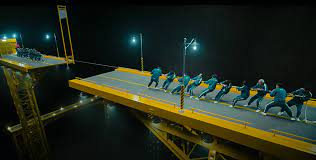
\includegraphics[width=0.75\textwidth]{images/tugofwar.jpg}
\end{center}

Remember that here, when we talk about concurrency, we mean two transactions that are ``active'' at the same time.

\end{frame}

\begin{frame}
\frametitle{Lost Updates}
Usually, we do not like to just allow both transactions to go forward because the first write is then overwritten by the second.

That is called a \alert{lost update}. 

This is sometimes  acceptable as a choice, even if some textbooks say that this is really undesirable and horrible.


\end{frame}


\begin{frame}
\frametitle{First Committer Wins}
The first snapshot isolation strategy is called \alert{first committer wins}.

Whichever transaction $T$ is ready to commit first has to pass a simple test. 

If any transaction concurrent with $T$ has already written an update to any data item that $T$ wants to write, $T$ is rolled back. 


Otherwise $T$ commits and its updates are written to the database. 


\end{frame}


\begin{frame}
\frametitle{First Committer Wins}

It's called first committer wins, because whatever transaction gets to the commit statement proceeds and any later transactions are rolled back.

\begin{center}
	
\includegraphics[width=0.3\textwidth]{images/good-day-sir.jpg}
\end{center}

\end{frame}

\begin{frame}
\frametitle{First Updater Wins}

The alternative is \alert{first updater wins}.

It is the timing of the write rather than the timing of the commit that indicates which transaction is allowed to proceed and which one(s) must be rolled back.  


\end{frame}

\begin{frame}
\frametitle{Locking and Unlocking}
Locks are always released when the transaction either commits or aborts.

A transaction $T_{2}$ writes a value later than $T_{1}$ writes that same value might actually succeed if for some other reason the first transaction aborts. 

But to keep things from getting rather confusing it is likely a simple implementation will just force the abort of $T_{2}$.


\end{frame}


\begin{frame}
\frametitle{Serializability}
This scheme as presented, however, does not ensure serializability.


Example 1: Concurrent transactions $T_{1}$ and $T_{2}$ that operate on $A$ and $B$. 

If $T_{1}$ reads $A$ and $B$, then updates $B$ and $T_{2}$ reads $A$ and $B$ and updates $A$, we have the potential for a conflict. 


\end{frame}


\begin{frame}
\frametitle{Serializability}

Neither transaction sees the updates of the other when they do their reads. 

When it comes to the write... well... 

Neither transaction is detected as conflicting and neither is rolled back.

\begin{center}
	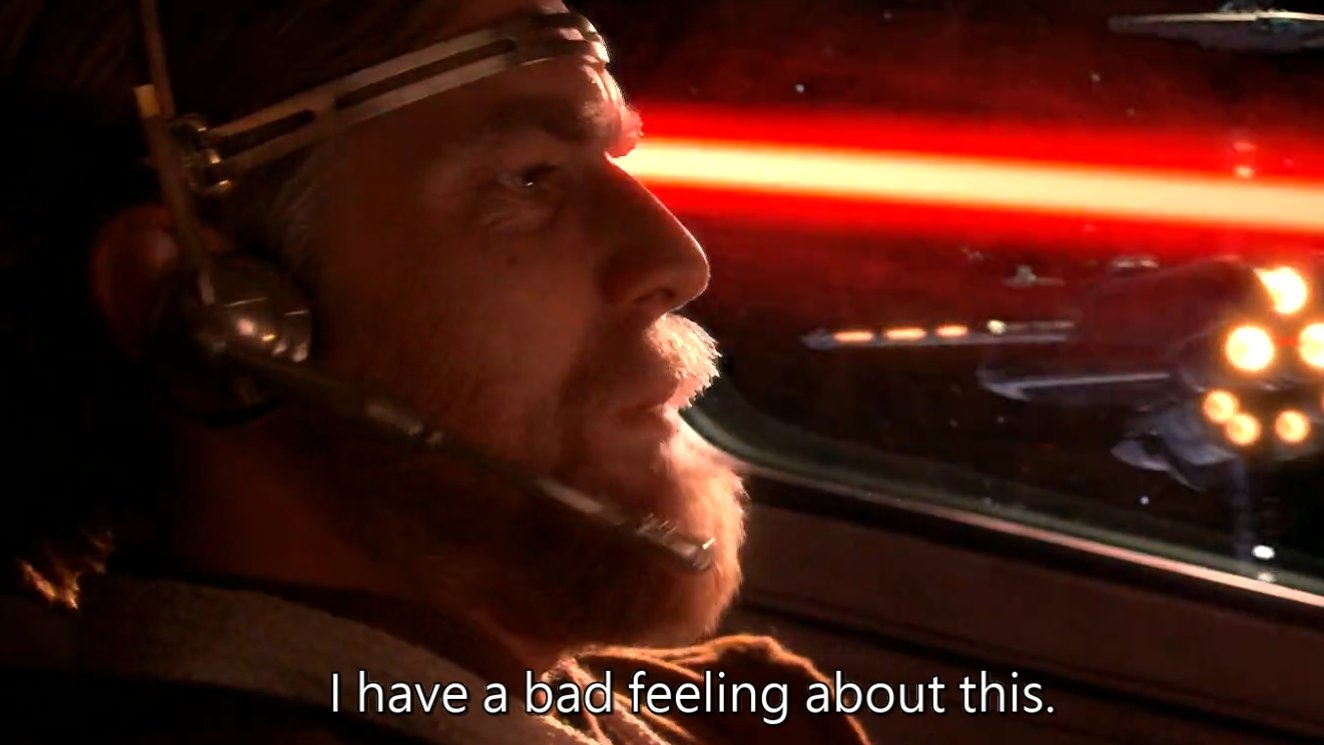
\includegraphics[width=0.5\textwidth]{images/badfeeling.jpg}
\end{center}

\end{frame}

\begin{frame}
\frametitle{Serializability}
In spite of that, we have a problem! 

We have an outcome (output data) that could not happen if we had serial execution of the transactions.

It looks like under this scheme, some things like foreign key checks, primary key checks, et cetera, cannot be checked in the transaction world itself.

They must be checked an extra time when the transaction commits and is finally ready to replace the actual stored version on the database.

\end{frame}

\begin{frame}
\frametitle{Serializability}
Imagine we still have $T_{1}$ and $T_{2}$ and $A$ and $B$ as before. 

$T_{1}$ reads $B$ and updates $B$, and $T_{2}$ reads $A$ and $B$ and updates $A$. 

As before, there are no direct conflicts on the data items so neither first-committer-wins nor first-updater-wins would detect a problem. 

\end{frame}

\begin{frame}
\frametitle{Serializability}

Furthermore, there's a possible serial order here: there are no conflicts on $A$, and no cycle in the precedence graph: 

$T_{2}$ reads the value of $B$ that existed before the write by $T_{1}$.

\end{frame}

\begin{frame}
\frametitle{A Wild Transaction Appears!}

\begin{center}
	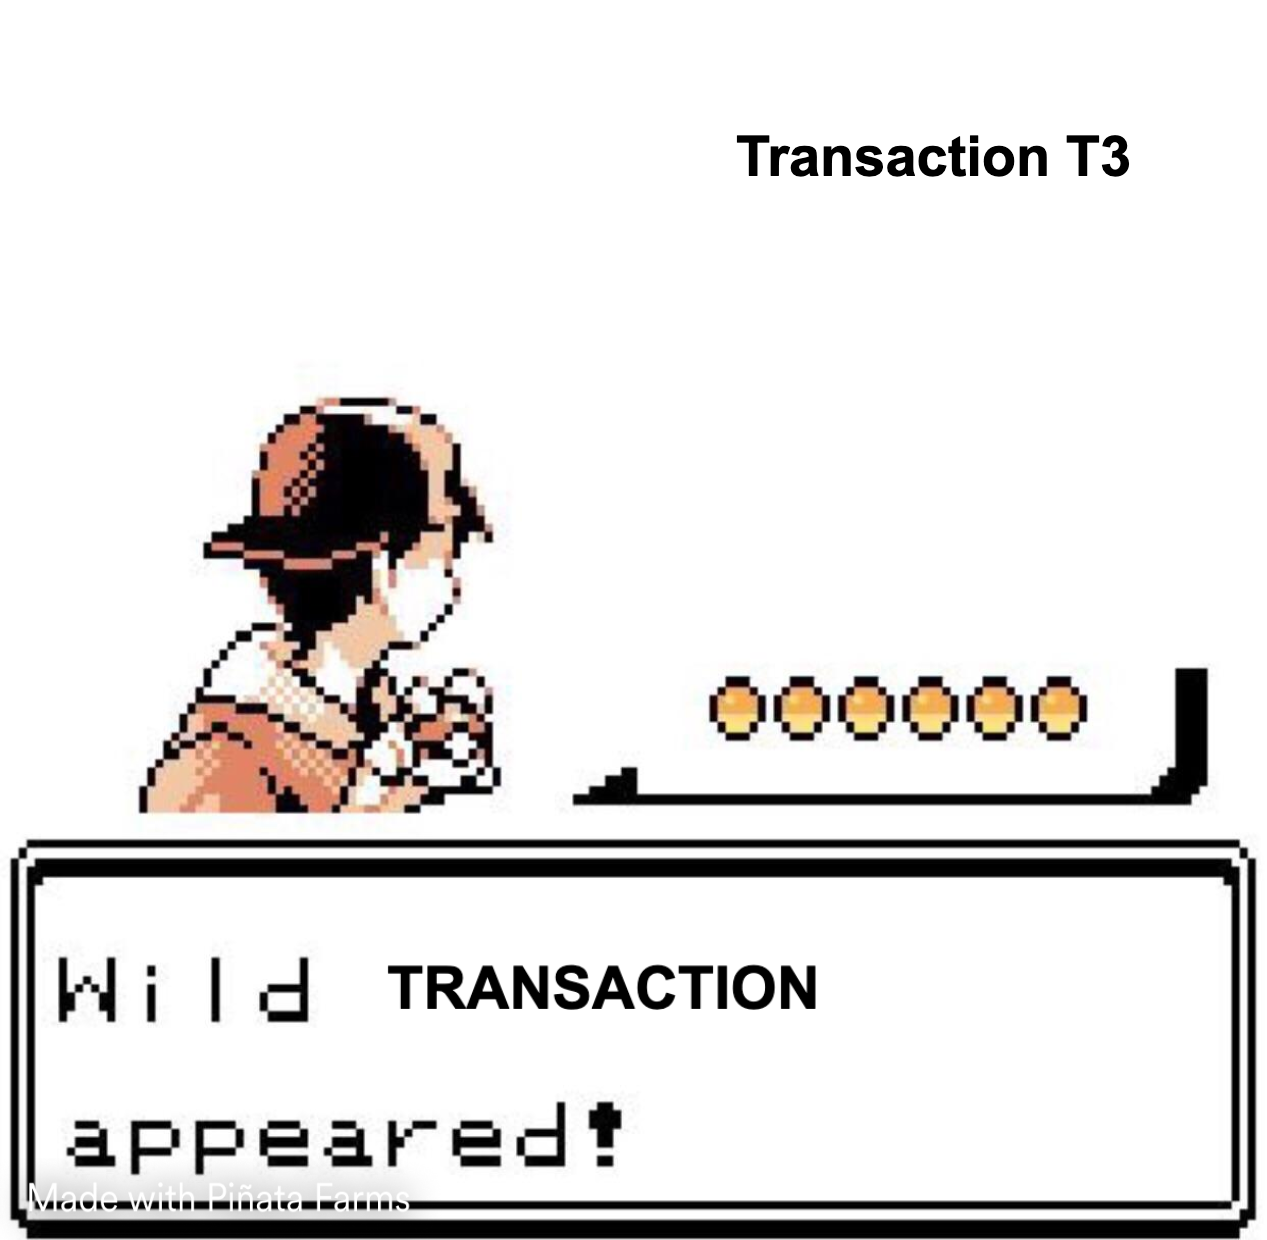
\includegraphics[width=0.7\textwidth]{images/t3.png}
\end{center}

\end{frame}

\begin{frame}
\frametitle{A Wild Transaction Appears!}

A third transaction, even one that is read-only, can cause the cycle to occur. 

If $T_{1}$ commits and $T_{2}$ is still running, and $T_{3}$ is created and its view of the world has the update from $T_{1}$ but not $T_{2}$...

We have the cycle in the precedence graph, making it non-serializable.


\end{frame}

\begin{frame}
\frametitle{Just Get It Done!}

After all that, though, we can accept some degree of non-serializability as long as it does not produce inconsistent results. 

For performance and other reasons it might be sensible to just let execution orders that are not serializable proceed.  

Or we will allow such things if we are convinced that inconsistencies don't make a big difference. 


\end{frame}

\begin{frame}
\frametitle{Key Constraints}
We might have to really enforce constraints: the primary key. 

If you have a sequential counter of some sort, an ID number, then two newly created entries could produce the same new number. 

Neither transaction can detect that another tried to use the same ID number. 

Only when we are actually ready to perform the second commit will the duplicate key value be detected.


\end{frame}

\begin{frame}
\frametitle{Insertion and Deletion}

All the discussion thus far on the subject of concurrency control has excluded the possibility of performing an insertion or deletion on the data items. 

Only read and writes were allowed. 

But those are pretty important operations, so we can't ignore them forever. 


\end{frame}

\begin{frame}
\frametitle{Deletion}

The impact of delete depends on what the else is going on at the time. 

We can take a view of what happens by considering the relation of the delete instruction relative to other instructions. 

The delete operation requires an exclusive lock on that data item.

\end{frame}


\begin{frame}
\frametitle{Deletion}

Cases to consider:

\begin{itemize}
	\item \textbf{Read instruction}
	\item \textbf{Write Instruction}	
	\item \textbf{Delete Instruction}
	\item \textbf{Insert Instruction}
\end{itemize}


\end{frame}

\begin{frame}
\frametitle{Insertion}

The insert operation conflicts were explained above when discussing deletion, so they don't need to be repeated here. 

Insert is also like a write, so again, the insert operation is treated like a write. 

The newly created item is treated as exclusively locked by its creating transaction until the transaction commits.

\end{frame}

\begin{frame}
\frametitle{Perspective}

At this level that the changes we want to make here are at the level of actual manipulation of the underlying data. 

It is perfectly valid, from the perspective of the user writing the SQL, to do a read and get back ``no results'' because the item was very recently deleted. 

The problem here is that we have identified what data elements we need to access and the ones we want are not there.

\end{frame}

\begin{frame}
\frametitle{The Phantom of the Op... Database}

\begin{center}
\includegraphics[width=0.7\textwidth]{images/phantom.png}
\end{center}


\end{frame}

\begin{frame}
\frametitle{The Phantom of the Op... Database}

Suppose the following transactions are executed concurrently: 

(1) a select statement that finds all books published by author ``Jim Butcher''; 

(2) an insert statement that adds a new book with author ``Jim Butcher'' amongst its attributes. 

\end{frame}

\begin{frame}
\frametitle{Sing Once Again With Me / Our Strange Duet}

There are two possibilities for how this might go: 


If $T_{2}$ happens first, nothing weird happens -- in the serial schedule, first it's $T_{2}$ then $T_{1}$ and the new book appears in the results. 

In the second case, if $T_{1}$ goes first and it does not contain the new book, then in the serial schedule, $T_{1}$ appears first... 

\end{frame}

\begin{frame}
\frametitle{Sing Once Again With Me / Our Strange Duet}

Except... these transactions do not operate on any tuples in common and yet there is still some dependencies between them. 

They conflict on a ``phantom'' tuple (one that doesn't exist). 

This is called the \alert{Phantom Phenomenon}

\end{frame}

\begin{frame}
\frametitle{My Power Over You / Grows Stronger Yet}
The phantom phenomenon can also happen if a read changes the value. 

If an item was entered incorrectly as ``Jim Butchr'', a corrective update statement run at the same time as $T_{1}$ above produces the same problem.

As a first solution, you might consider that an insertion or deletion should exclusively lock the relation entirely.

This can work but is very painful!

\end{frame}

\begin{frame}
\frametitle{And Though You Turn From Me / To Glance Behind}

Remember the index? 

So far we have just assumed that data items being updated are tuples, but that's not strictly true, because index data elements also need to be lockable.

Idea: let's associate a data item (available to be locked) with each table, with the goal that it represents the way to find tuples in the relation.

\end{frame}


\begin{frame}
\frametitle{The Phantom of the Database Is There}

To update the data about what is in the relation, and transactions that want to read what tuples are in the relation need to also lock this item. 

And anything that operates on an index must lock the index. 

This moves the lock out of the realm of shadows and into the ``real'' world -- the lock conflicts here are now on an actual lock item.


\end{frame}

\begin{frame}
\frametitle{Inside Your Mind}

Keep in mind this is very much distinct from locking the entire table. 

Holding this sort of lock only restricts whether other transaction can update (or read) the information about what tuples are in the relation. 

Even so, it's not all that dissimilar from the idea of having one lock for the whole table, in that it almost serializes all transactions.

An alternative is \alert{index locking}, which allows us to lock parts of the index.

\end{frame}



\begin{frame}
\frametitle{He's There, The Phantom of the Database}

\begin{itemize}
	\item Every relation must have at least one index.
	\item A transaction $T_{i}$ can only access tuples after it has found them using an index.
	\item A transaction that performs a lookup (finding one tuple or multiple) must get a shared lock on all the index leaf nodes it accesses.
\end{itemize}
	
	\end{frame}



\begin{frame}
\frametitle{He's There, The Phantom of the Database}

\begin{itemize}
	\item A transaction may not insert, delete, or update any tuples in the relation without updating every index of that relation. That requires getting exclusive locks on all index leaf nodes affected by the operation. 
	\item Locks are still obtained on tuples as usual.
	\item Two phase locking protocol still must be followed. 
\end{itemize}


\end{frame}

\begin{frame}
\frametitle{Predicate Locking}
You may imagine that the idea of index locking does not actually match very well with the idea of making the locking match the predicates only.

Example: only checking on things that affect author. 

That technique sounds good but it is more difficult to implement. 

\end{frame}

\begin{frame}
\frametitle{Weak Consistency}

The SQL standard provides several isolation levels, and it's not necessary that we stick with serializability as the level of consistency we are willing to accept. 

We can weaken the rules a bit to get some more performance out of the database and that gives us what is called \alert{weak consistency}. 

\begin{center}
	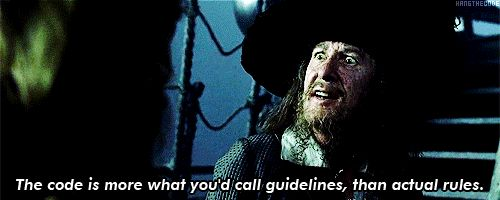
\includegraphics[width=0.6\textwidth]{images/barbosa.jpg}
\end{center}

\end{frame}

\begin{frame}
\frametitle{Degree-Two Consistency}

The idea of \alert{degree-two consistency} is to prevent cascading rollbacks (aborts) without guaranteeing serializability. 

There are shared and exclusive locks, but two-phase behaviour is not required. 

Shared locks can be released at any time and locks can be acquired at any time, but exclusive locks must be held until the transaction commits or aborts. 

This means that we might read out of date data, but uncommitted values can never be read, so the level of transaction isolation here is ``read-committed''.
 
\end{frame}

\begin{frame}
\frametitle{Cursor Stability}

Cursor stability is a form of degree-two consistency for programs that iterate over some set of tuples using an iterator or cursor. 

The tuples are examined or processed one at a time, in some order. 

The tuple currently being examined needs to be locked: before processing it is locked in shared mode. 

If any processing changes that tuple, it must first be locked in exclusive mode. 

\end{frame}

\begin{frame}
\frametitle{Cursor Stability}

We don't get serializability of the transactions. 

It can be a way to improve performance in a database where there are a number of relations that are popular and frequently accessed. 

This offloads some of the work onto the applications using the database. 

They must be sure they don't have a problem with non-serializable schedules.


\end{frame}

\begin{frame}
\frametitle{Users Ruin Everything...}

Remember the example earlier about selecting seats on a flight?

\begin{center}
	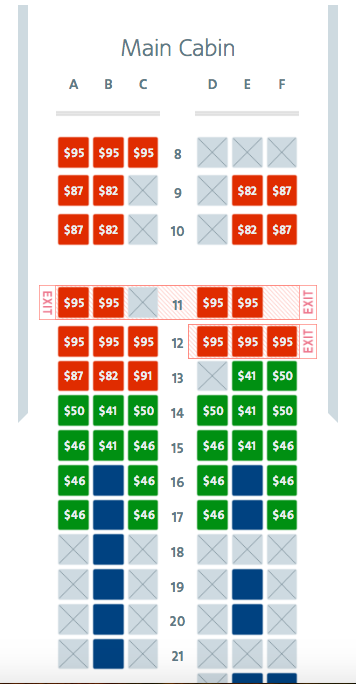
\includegraphics[width=0.3\textwidth]{images/seat-selection.png}
\end{center}

\end{frame}

\begin{frame}
\frametitle{Users Ruin Everything...}
You have some period of time, e.g., 2 to 10 minutes to get this done. 

That is a very long time as far as the database is concerned. 

If two transactions select the same seats then we reject the second transaction.

\end{frame}


\begin{frame}
\frametitle{Users Ruin Everything...}

This has a major drawback when we're dealing with user-level timeframes. 

The database must remember information about updates performed by a transaction long after it has ended... 

For as long as any other concurrent transaction is still alive.

In the case of transactions like a booking that give you 10 minutes of time, this means a transaction's information needs to be retained for up to 20 minutes. 


\end{frame}

\begin{frame}
\frametitle{Split 'em Up}

A more likely solution is that we need to split it up into multiple transactions. 

One transaction is completed to read the data and it is provided to a client application (e.g., web browser). 

Then another transaction is needed when the user is ready to save changes: we create another transaction to save the data back to the database. 


\end{frame}

\begin{frame}
\frametitle{In The Upside Down}

The data may have changed in the meantime, and if they did the attempt to merge the changes in that transaction will result in an error. 

What the application needs to do is reload the data (repeat the read(s) that produced the data elements and see if they changed. 

Detecting changes isn't as simple as just comparing fields, because it (1) would require saving the original read version, and (2) the ABA problem.

\end{frame}

\begin{frame}
\frametitle{ABA Problems}

The solution to the ABA problem is version numbers: every tuple is assigned a number that represents the version. 

It is initialized to 0 and incremented (atomically) each time the tuple is updated. 

Then a transaction needs only to look at the version number. 

If the version number doesn't match the original read, then it has changed.
\end{frame}


\begin{frame}
\frametitle{Holy Long Names Batman!}
This is called \alert{optimistic concurrency control without read validation}. 

We assume we are going to succeed without conflict (are optimistic) and rollback if we must. 

It is without read validation, because we check version numbers only for writes that we are going to perform. 

If we want optimistic concurrency control, then we must also check the version numbers of any reads that went into the transactions too.

\end{frame}

\begin{frame}
\frametitle{Concurrency in Index Structures}

We can use special handling for the index structures to improve performance. 

Allow non-serializable access to the index as long as the results are consistent. 


\end{frame}

\begin{frame}
\frametitle{Crabbing Protocol}

The first technique for locking on index structures is the \alert{crabbing protocol}.

\begin{center}
	
\includegraphics[width=0.4 \textwidth]{images/crab.jpg}
\end{center}

When searching for a key value, first lock the root note in shared mode. 

When traversing down the tree, acquire a shared lock on the child node and release the lock on the parent node, repeating this until a leaf node is reached.

\end{frame}

\begin{frame}
\frametitle{Crabbing Protocol}


When performing an insertion or deletion of a leaf node:
\begin{itemize}
	\item Follow the same protocol to reach the leaf node (acquire and release shared locks).
	\item Lock the leaf node in exclusive mode and perform the insertion or deletion.
	\item If a split or coalescence is needed, lock the parent in exclusive mode and do the changes; release the leaf nodes.
	\item If the parent itself needs splitting or coalescing, retain the lock on the parent and propagate the changes; otherwise release the parent.
\end{itemize}


\end{frame}

\begin{frame}
\frametitle{B-Link Trees}
The second technique we will talk about requires a modification of the B$^{+}$-trees called \alert{B-Link} trees. 

These have the added restriction that says every node (really, all of them) have a pointer to its sibling to the right. 

This helps in case a search is taking place at a time when a node is being split and it can continue. 


\end{frame}

\begin{frame}
\frametitle{B-Link Lookup}

Each node must be locked in shared mode before it is requested. 

A lock on any non-leaf node is released before a lock on any other node is requested. 

If a split takes place while a lookup is happening, then we might need to look in the sibling to find something. 

Leaf nodes are locked using the two phase protocol.

\end{frame}

\begin{frame}
\frametitle{B-Link Insertion/Deletion}

The rules for lookup are followed to find the leaf node where the records will be inserted or deleted. 

The lock for the leaf is upgraded to exclusive; insertion or deletion is performed. 

Two phase locking is used to avoid the phantom phenomenon.

If as a result of insertion or deletion, a split or coalescence is needed...

\end{frame}

\begin{frame}
\frametitle{B-Link Split}

If a node is split, a new node is created as per normal for a B-Tree and it becomes the right sibling of the original node. 

The previous right sibling of the original is the right sibling of the new node. 

Then the original node is released and an exclusive lock on the parent is requested to insert a pointer to that new node.

\end{frame}

\begin{frame}
\frametitle{Coalescence}

If a node need to be coalesced, then the node it will be merged with must be locked in exclusive mode. 

Then the parent node of the newly-created node must be locked exclusively so that the deleted node can be removed. 

The parent may be coalesced as well if necessary, otherwise it is released.

\end{frame}

\begin{frame}
\frametitle{B-Link Chemistry}

\begin{center}
	\includegraphics[width=0.9\textwidth]{images/b-link1}
	\vspace{5em}
	\includegraphics[width=0.9\textwidth]{images/b-link2}
\end{center}


\end{frame}

\begin{frame}
\frametitle{B-Link Chemistry}

Let's see what happens if there is a lookup while this is going on.

The lookup gets blocked at the bottom-left leaf node because it is exclusively locked by the insertion. 

The lookup holds no locks at this point.

What if instead of a split there was a coalescence?

\end{frame}



\begin{frame}
\frametitle{Key-Value Locking}

Key-value locking allows locking individual key values, allowing other operations to take place on values within the same leaf node.

The problem is that we could still have the phantom phenomenon, so the strategy of \alert{next key locking} is employed. 

Not only lock the keys that are in the range/search result but also whichever one is next. 

This prevent something from being inserted, altered, or deleted inside the search range. 


\end{frame}









\end{document}

